\providecommand{\mainpath}{..} % Command to retrieve the path of the main file. It must be defined before documentclass.

\documentclass[\mainpath/main]{subfiles}
\begin{document}

\chapter{Architectural Design}
\label{architectural_design}

% Command to be executed after the starting of every chapter
\setmyfancystyle
% ----------------

In this chapter the complete architecture of myTaxiService is shown with various levels of description. In the \autoref{ArchitecturalDesign:high_level} there is a global view and the interactions between all the components are described.\\ 
The data tier is illustrated in \autoref{ArchitecturalDesign:component} with all related policies and entities. Then the other tiers are characterized using different diagrams.\\
In the \autoref{ArchitecturalDesign:deploy} the deployment of each components is illustrated (for instance the data component is sit in a different place with respect to the other component? It is replaced twice or more? And similar question will have an answer).\\
In \autoref{ArchitecturalDesign:runtime} the view level is defined. The interactions between all kinds of user and the system are described using UX diagrams and sequence diagrams that display the order in which each screen is visualized. Besides, the \glspl{mockup} of these screens are shown in \autoref{UIDesign}.
\\
A standalone paragraph, the \autoref{ArchitecturalDesign:comp_interfaces}, is dedicated to list all interfaces, both internal (between two components) and external.\\
Finally, in the \autoref{ArchitecturalDesign:design_patterns} the design patterns used to develop myTaxiService are described first in general case. After that, all the changes needed to adapt this design patterns to our system are characterized.


\section{Distinctions between various kind of Users and Clients}
\label{ArchitecturalDesign:preamble}
The "visible architecture" of myTaxiService is very varied. The term visible is referred to various user interfaces, so what the users can see when they are using the system.\\
On the other hand, we have said that myTaxiService is varied because it has two principal version (\gls{ma} and \gls{ws}) and for both of them there are a few levels of specialization, according to the kind of the user. All of them are explained in this paragraph.\\
\\
The WS version is shown into a browser, so there is no client application that can be used. Hence, all the pages are loaded into the server and then they are sent to the client browser.\\
Instead, the \gls{ma} is a client application and it has different ways to communicate with the server. All the aspects concerning these differences are explained better during the descriptions of the architecture's components that handle the clients.\\
\\
%Fare un riferimento al capitolo che mette in relazione RASD e DD per far capire il tipo di attore?
The cab company is the special user who administrates the service. Obviously, it has a command center at its headquarters where it can control both the system and the service situation. Hence its special functions are not implemented neither in the \gls{ma} nor in the \gls{ws}, but they can directly access the server using private keys and reserved terminals.\\
A customers can use both the \gls{ma} and the \gls{ws} to enjoy his functionalities. No particular cases or restriction are reserved to them.\\
When a driver logs into the service, we suppose that it is working, so his special functionalities are developed and implemented only for the \gls{ma}. In fact no driver carries a computer with an internet connection on his taxi and uses it. On the other hand, since the driver is also an user, it can use the WS, but here he has only the user functionalities due to the reason shown above.\\



\section{High level components and their interaction}
\label{ArchitecturalDesign:high_level}

The main structure of myTaxiService can be described as a Service-Oriented architecture (see \autoref{ArchitecturalDesign:design_patterns} to have a detailed description of this design pattern). In addition to this idea the Model-View-Controller paradigm is applied in order to develop a good-programmed, reusable and easy-maintainable system.
\begin{figure}[h]
	\centering
	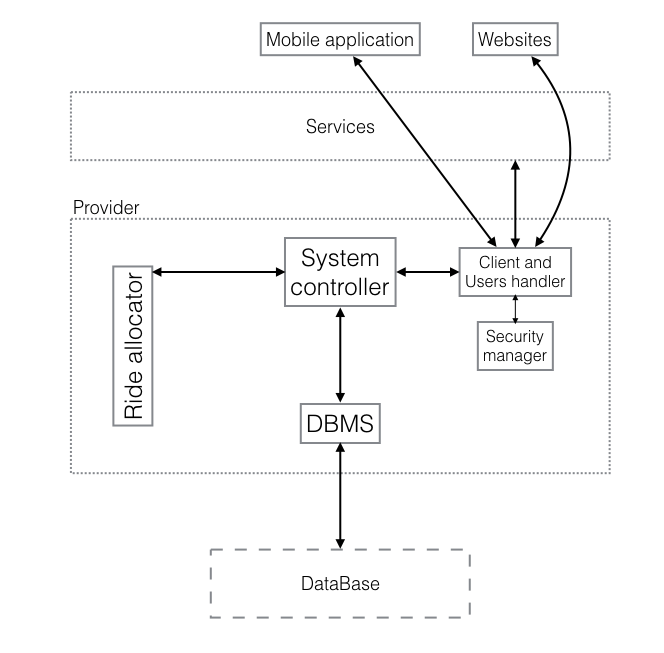
\includegraphics[width=10cm] {main_architecture}
	\caption{High level architecture}
	\label{ArchitecturalDesign:figure1}
\end{figure}

In the figure \ref{ArchitecturalDesign:figure1} is shown the architecture. At the bottom of the figure there is the \nameref{ArchitecturalDesign:datatier} which contains only the database (a component that stores all data about the customers, the rides and the system).\\
\\
The central part of the picture contains the provider, the big component that gives the service. At this level of description we can look in the provider. This component is split into five parts. The DataBase Management System (DBMS) manages all communications with the \nameref{ArchitecturalDesign:datatier}. The Ride Allocator has only one role, to assign and to handle the ride, both future and zerotime. The system controller is the \textquotedblleft heart\textquotedblright of the provider: it involves the ride allocator when is needed, it gives all the services of the system, it provides the DBMS with the data to be stored (or asks him some data to be found) and communicates with the Client and Users Handler. The Client and User Handler, as its name said, handles the communications with the clients and administrates the Users, so which services can be shown and selected by them.\\
\\
The third tier is a presentation level. In the Service-Oriented pattern this level represents the available services. Here, the clients can see the services and select the desired one.\\
Finally, at the top of the image, there is a representation of the two kind of clients, the \gls{ws} and the \gls{ma}.\\
\\
All the tiers are also distinguished into the three parts of MVC-paradigm. The \nameref{ArchitecturalDesign:datatier} is the model\footnote{see the Alloy section or the UML class diagram into the RASD to see it. However, in section \ref{ArchitecturalDesign:datatier} it is studied again.}. The provider is also the controller: even if the controller can be seen as the component that manages the interaction between the view and the model, in this application we consider other \textquotedblleft handler\textquotedblright as part of controller because they encapsulate rules and action codes. The view is the union between the presentation tier (here the services are only shown to client, the \textquotedblleft decisions\textquotedblright are taken by the provider) and the clients.\\
\\
Up to now, we have introduced all the main components or tier of our system, without focusing on the communications between them, so we'll dedicate a little part of this paragraph on this argument.\\
All the communications between the model and the provider are managed by the DBMS that has store policies and finds the required data. The system controller is the central node in communication because it is the only way to all the other components of the provider.
The Client and User Handler is the link between the provider and the clients. It checks the type of the current user and, as consequence, the available services that he can uses. When a user asks a service, he binds the request asking for the related function to the System Controller. Finally, it checks the type of client, because they have two ways of communication. When a user is connected with the WS, the Client and User Handler load the pages into itself and then, using the HTTPS protocol sent them to the client. Besides, the communications with the \gls{ma} is implemented using sockets. The implementation of these ways of communication with the clients is realized by a common interface (see the section \ref{ArchitecturalDesign:comp_interfaces} for further information).

\section{Component view}
\label{ArchitecturalDesign:component}


\subsection{Data tier}
\label{ArchitecturalDesign:datatier}

This paragraph shows the Logical schema of the database in figure \ref{ArchitecturalDesign:datatier_figure} for the application.\\
The tuples names are written in italic style, the underlined attributes are the primary keys, while the
bold attributes are the reference keys.\\
\begin{itemize}
	\item \textit{rides} (\underline{rideID}, \textbf{passenger}, \textbf{driver}, \textbf{departure}, \textbf{destination}, departureTime, arrivalTime, creationDate, isFuture) : \\
	it contains both the zerotime rides and future rides, the field isFuture has value 1 when it's a future ride, 0 when zerotime ride.
	
	\item \textit{users} (\underline{userID}, email, password, name, surname, taxcode, birthday, cityOfResidence, isDriver, registrationDate, activationCode, activated) : \\
	it contains the general and fundamental information of all the users. The field isDriver has value 1 when the user is a driver, 0 otherwise. The field activated has value 1 if the user has completed the registration process by confirming on the link with his activation code sent to his e-mail address, 0 otherwise.
	
	\item \textit{drivers} (\underline{driverID}, \textbf{userProfile}, cabCarCode, \textbf{cabCompany}) : \\
	it contains all the information of the drivers. The field userProfile is the reference key to the record in the users table which contains all the other general information of the driver.
	
	\item \textit{cabCompanies} (\underline{cabCompanyID}, name) : \\
	it contains all the cab companies that use myTaxyService.
	
	\item \textit{positions} (\underline{positionID}, gpsLatitude, gpsLongitude, \textbf{address}, civicNumber) : \\
	it contains the stored positions for the rides (departure and destination) with the reference to the corresponding address in the table addresses and optionally the gps coordinates and the civic number.
	
	\item \textit{addresses} (\underline{addressID}, city, street, \underline{area}) : \\
	it contains all the existing streets and cities covered by myTaxyService, with the reference to the area which they belong to.
	
	\item \textit{areas} (\underline{areaID}, name) : \\
	it contains all the areas covered by myTaxyService.
	
	\item \textit{driversWaiting} (\underline{\textbf{area, driver}}, driverAddedTime) : \\
	it contains all the available drivers waiting for a ride request. The couple of keys "area,driver" is unique because a driver cannot be available in more than one area at time. The field driverAddedTime contains the date and time when the driver is added to the list of available drivers for a certain area, it is useful to sort the list with the desired order (a FIFO queue in our application).
	
	\item \textit{workShifts} (\underline{workShiftID}, \textbf{driver}, weekDayNumber, startingTime, endingTime) : \\
	it contains all the work shifts of a driver. weekDayNumber is the number of the day of the week (between 1 and 7, 1 is Monday, 7 Sunday). startingTime and endingTime represent a continuous time range of a work shift of a driver in a certain day of the week.
	
	\item \textit{alerts} (\underline{alertID}, \textbf{user}, receptionDate, message) : \\
	it contains all the alerts that a user has received. "user" field is the reference to the receiver of the alert.
	
\end{itemize}

\begin{figure}[h]
	\centering
	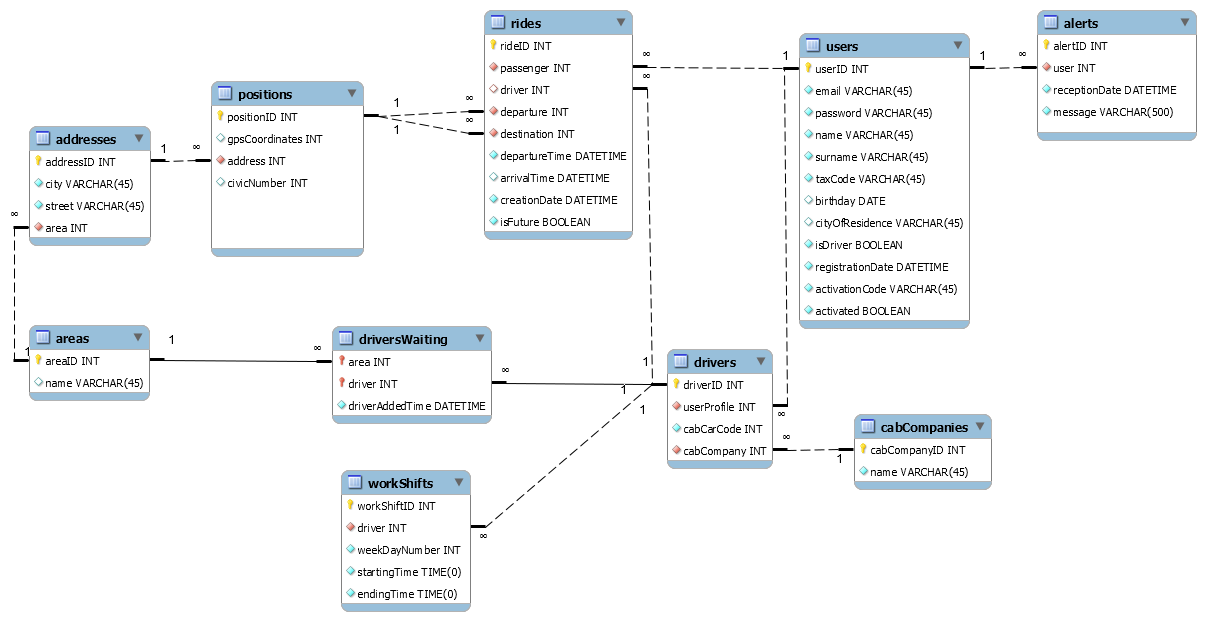
\includegraphics[width=0.75\paperheight, angle=90] {DataTier}
	\caption{Logical schema of the database in the Data tier}
	\label{ArchitecturalDesign:datatier_figure}
\end{figure}

\clearpage

\subsection{Provider tier}
\label{ArchitecturalDesign:provider}

The provider is the \textquotedblleft hearth\textquotedblright of myTaxiService and it is split into several components, each one dedicated to a specific function. In \autoref{ArchitecturalDesign:high_level} a short description of the provider's components has been written. In this paragraph we'll go in deep for each one.\\
The \textbf{DBMS}, as its name says, manages the database and gives the system an interface to search, update or delete data. This interface can be used only by the System Controller by the use of queries already written into the application code. When the DBMS receives a query, first checks it to prevent some malevolent data (for instance SQL injection on same parameter asked to the client), then performs the required operations and gives methods to access the result.\\
\\
The \textbf{Security Manager} is a small component that implements all the security procedures of the provider. It contains:
\begin{itemize}
	\item The definition of the data encryption methods;
	\item The firewall methods between the Provider and the Client and Users Handler;
	\item The HTTPS protocol implementation;
	\item The algorithms to check the authenticity of the administrators. \\
\end{itemize}

The \textbf{Client and Users Handler} binds the clients to the provider, so it has the following functions:
\begin{itemize}
	\item \textit{Client interface.} The handler implements the common interfaces of the clients\footnote{see \autoref{ArchitecturalDesign:comp_interfaces} to have a precise description of the interface.} to hide the kind of the client to the provider. In \autoref{ArchitecturalDesign:preamble} it is available a description of the main differences between the two client's versions.
	\item \textit{Authentication.} The handler implements the methods to recognize the type of user by a code automatically generated by the System Controller at each valid session (typically it is the cookie used by the user or a similar number if he is using the \gls{ma}).
	\item \textit{Services showing.} With the authentication module support the handler can decide which class of services can be seen by the user.
	\item \textit{Services interfaces} In this component the interfaces for each group of services (there is an hereditary hierarchy to realize them) are defined to allow the handler to bind the desired service by calling the System Controller (for security reason it is only possible to enqueue the request on the System Controller buffer). An other reason for their presence in this component it's the possibility to show that on the presentation tier.\\
\end{itemize}

The figure \ref{ArchitecturalDesign:clientAndUsersHandler} shows a simple class diagram that models the Client and User Handler, as it was described above.\\

\begin{figure}[h!]
	\centering
	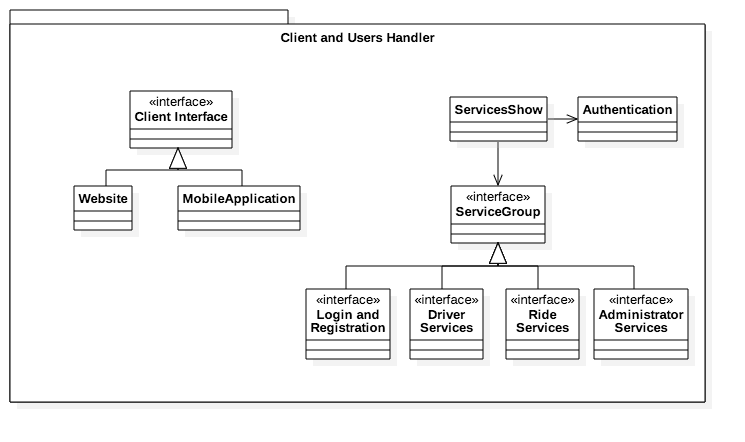
\includegraphics[width=\textwidth]{component/ClientAndUsersHandler}
	\caption{A class diagram for the Client and Users Handler.}
	\label{ArchitecturalDesign:clientAndUsersHandler}
\end{figure}

The \textbf{Ride Allocator} is a component involved by the System Controller only when a ride needs to be assigned and when a driver starts to wait for a new ride. Its functionalities are related to the situations described a few words before. The implementation of these functionalities is hidden to System Controller, that invokes them by an interface\footnote{In \autoref{ArchitecturalDesign:comp_interfaces} it is described this interface and the external interfaces used to implement the city map and the localization}.\\
First, the Ride Allocator creates a representation of the city map split into areas\footnote{An important remark on area division is the following. As it is partially described into data tier model, the division into the areas is not made by a set of positions. An area is composed by a set of streets that are closest to each other. This choice can create same strange areas when a street is very long: in this case the area is composed by a set of closer streets that defines a polygonal area and by a street that is include into this polygon, but \textquotedblleft fills out\textquotedblright for part of itself.}. With this representation and the external APIs it is easy to identify the area where either a position or an address is into.\\
Second, the Ride Allocator has to manage the queues for each areas, so it has two subcomponents dedicated to this purpose: the Queue Creator which creates and defines a queue for each area; the Queue Manager that implements the methods to handle the queues, so the management policies, the adding or the removing of a driver and so on.\\
Finally, the Allocator assigns a cab-man to a ride for which the starting position (the destination is only an information for the driver, but not for this component) is passed by the System Controller.\\
In figure \ref{ArchitecturalDesign:rideAllocator} the Ride Allocator is modelled by a simple class diagram.\\

\begin{figure}[h!]
	\centering
	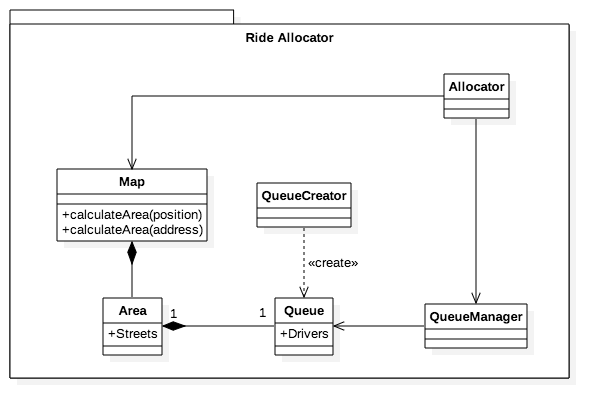
\includegraphics[width=0.75\textwidth]{component/RideAllocator}
	\caption{A class diagram for the Ride Allocator.}
	\label{ArchitecturalDesign:rideAllocator}
\end{figure}

The \textbf{System Controller} is the central node of the application: all the communications pass through it. As consequence it requires a very good design to not slow down the system.\\
The main subcomponent is the Dispatcher, realized first as an interface with only the method to enqueue a request for another component (for instance an user request coming from the Client and Users Handler), then as a concrete implementation with all the hidden methods. The requests are also handled. The policy to manage the request is a three priority levels FIFO\footnote{FIFO means \textit{First In First Out}, so the first arrived request is handled before the others. In addition there are three priority levels to allow a more important message to be handled earlier than a low-priority one arrived in advance.} queue, where the first level is reserved to some problems that can occur during system execution and the second one is dedicated to the administrators' operations. To clarify, near the 100\% of the message have the low-level priority, but the system is able to immediately react when a fault or an external attack happen (the related messages have the high-level priority).\\
Second, the User Creator is able to create user by Factory Method pattern\footnote{see \autoref{ArchitecturalDesign:design_patterns} for a formal description of this design pattern.}. Hence, with some strategies hidden by that pattern the User Creator creates the correct type of user. This fact implies an important consequence to the system: each type of user can create or not particular cookies to allow the Client and User Handler to recognize them and to perform the available operations.\\
Third, the User Checker is a supplementary component to increase the security of the system and works in parallel to the Dispatcher. When a request is enqueued to the dispatcher low-level the Checker immediately checks the validity of that request and, if any, the request is removed by the queue.\\
Fourth, the Data Checker has the only role of checking the validity of input data inserted by an user. Thus, it checks the correctness of inserted addresses (in collaboration with the Ride Allocator) and of personal data.\\
Finally this component contains all the main logic of the system, so all the classes not related to some particular component (for instance all the handlers and the rides' definition and management) is defined here.\\
In figure \ref{ArchitecturalDesign:systemController} a class diagram that model this component is shown.

\begin{figure}[ht!]
	\centering
	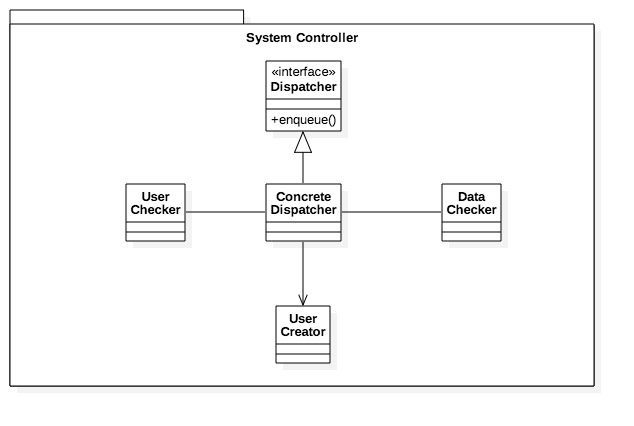
\includegraphics[width=\textwidth]{component/SystemController}
	\caption{A class diagram for the System Controller.}
	\label{ArchitecturalDesign:systemController}
\end{figure}

%\clearpage

\subsection{Presentation tier}
\label{ArchitecturalDesign:services}

The available services are grouped into four main section:\\
\begin{itemize}
	\item \textit{Login and Registration.} This service is always available at the first access to myTaxiService, both for the \gls{ma} and the \gls{ws}. The user (it is not important which kind of user he want to become) has to log into the service or to register himself the first time. When the visitor clicks on login \footnote{see \autoref{UIDesign} for further information}, he inserts his personal keys, then the Client and User Handler verifies the correctness of those keys, then checks the type of user to shows his services. (If the user is a driver or a cab company administrator other special credentials will be asked to increase security).\\
	
	\item \textit{Ride services.} This macro section contains all the functionalities related to the rides, so the characteristic ones of myTaxiService. The zerotime and future rides' reservation, the possibility to view or to modify the personal rides and the reading of user's alerts belong to this area and they are all shown together.\\
	The Client and User Handler shows these services to all logged users (except for the administrators).\\
	
	\item \textit{Driver services.} Driver services is a section reserved to the drivers logged into the \gls{ma}, for the reason presented in \autoref{ArchitecturalDesign:preamble}. The functionalities give here are the management of work shifts, the notifications of availability and the reading of reserved alerts (for instance, the request for a ride or the confirmation of a ride).\\
	
	\item \textit{Administration services.} This section, for security reasons, can be accessed only with administrator credentials (they consists in a couple name and password and in the use of an electronic card) into the company's headquarters on the \gls{ws} version. The Client and User Handler shows into this section the following functionalities: create or remove a driver profile, notification for all the users (usually, for general information or problems with the service) and checks some service information (for instance anomaly values of taxi queues).
\end{itemize}


\section{Deployment view}
\label{ArchitecturalDesign:deploy}

In this section the deployment of myTaxyService is pointed out.
Due to the reasons explained in \autoref{ArchitecturalDesign:provider} the most important component of the system is the Dispatcher, thus this component has a half of the computational power of the system dedicated only to itself. The other components of the provider are located in the same physical location of the System Controller unit, but on various nodes, according to this guide line:\\

\begin{itemize}
	\item the remaining computational power is equally distributed among four other nodes;\\
	\item the Ride Allocator and the subcomponents of the System Controller (except for the Dispatcher) are sit in the same node;\\
	\item the DBMS and the Client and Users Handler are located on standalone nodes.\\
\end{itemize} 

Figure \autoref{ArchitecturalDesign:deploymentFigure} shows a deployment diagram that focuses on the communications between significant nodes and on the presence of the nodes themselves.

\begin{figure}[ht!]
	\centering
	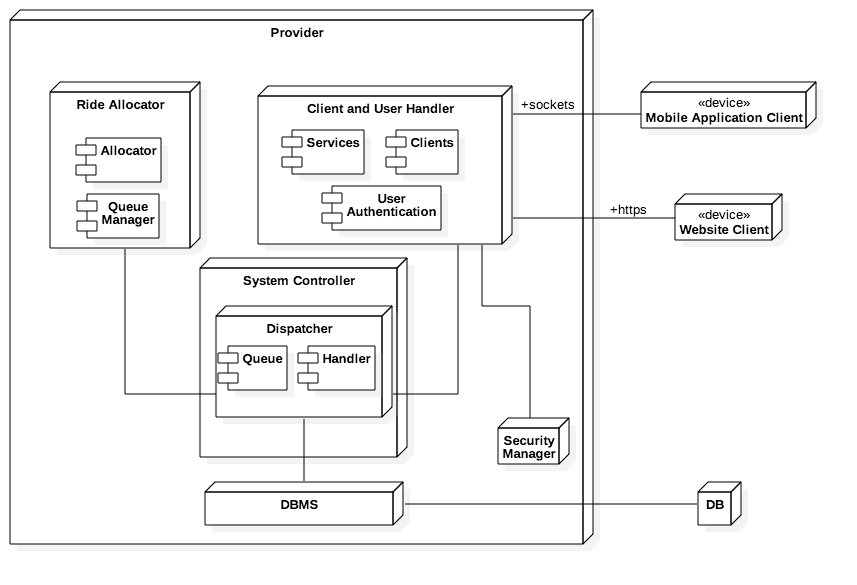
\includegraphics[width = \textwidth] {DeploymentDiagram}
	\caption{A deployment diagram for myTaxiService.}
	\label{ArchitecturalDesign:deploymentFigure}
\end{figure}

In addition to this short description, two firewalls are located to improve security: one out of the Provider (the communication links outgoing from the Client and User Handler to the Clients) and one on the communication link between the Dispatcher and the Client and User Handler.\\
At last, in figure the database is represented as a node: into the designed architecture the database is replaced twice to prevent loss of data and these two portions are located in different places with respect to each other and to the physical location of the provider architecture. To be precise these two position are into a circle with radius fifty kilometres and centre on the provider's location. The policies related to access the database, to store and to backup all the data (into other location) are defined by the DBMS, that communicate with the two database thanks to an encrypted connection.

\section{Runtime view}
\label{ArchitecturalDesign:runtime}

In this paragraph we'll show the main features on the runtime view, which means the UX diagrams and the sequence diagrams.\\
The UX diagrams display the structure of the myTaxiService's screens (input forms, available functions and shown data) and the effects of each function (the next screens viewed). The sequence diagrams show the sequence of functions' calling and screens to benefit of a functionality.\\
\\
An important note is the following: the functionality Read The Alerts\footnote{see the RASD for further information.} is not shown here. It is performed as a simple screen on the Homepage that redirect to another screen with only the list of alerts (composed by a title and a written text).\\
\\
Finally, the two version of myTaxiService (\gls{ws} and \gls{ma}) have no differences on the visualization of the screen. In fact, the screen has the same name and the same purpose, but they are adapted to the particular version where they are displayed.\\
In particular, the sequence diagrams are usually referred to the \gls{ws} version to define the labels of each arcs, but the same labels can easily \textquotedblleft translated\textquotedblright to the \gls{ma} version. For instance, in figure \ref{ArchitecturalDesign:SD_Registration} the first edge has as label \textquotedblleft \textit{navigate to myTaxiService websites}\textquotedblright . In the \gls{ma} this sentence is equivalent to \textquotedblleft \textit{open myTaxiService's application}\textquotedblright .

%\clearpage

\subsection{UX Diagram}
\label{ArchitecturalDesign:UX}

\subsubsection{Starting Page}
\label{ArchitecturalDesign:UX_StartingPage}

\begin{figure}[hb!]
	\label{ArchitecturalDesign:firstUX}
	\centering
	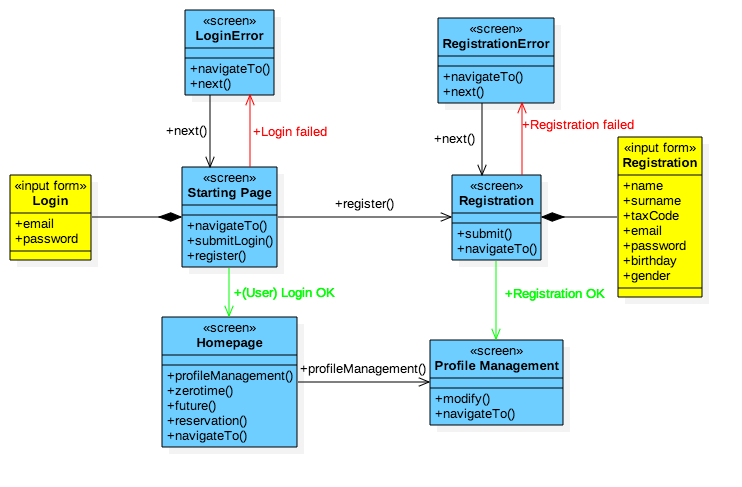
\includegraphics[width = \textwidth] {runtime/UX_StartingPage}
	\caption[UX Diagram from the Starting Page.] {The UX diagram from the Starting Page. The main functionalities available from this screen are displayed here.}
\end{figure}

\clearpage

\subsubsection{Profile Management}
\label{ArchitecturalDesign:UX_Homepage}

\begin{figure}[hb!]
	\label{ArchitecturalDesign:secondUX}
	\centering
	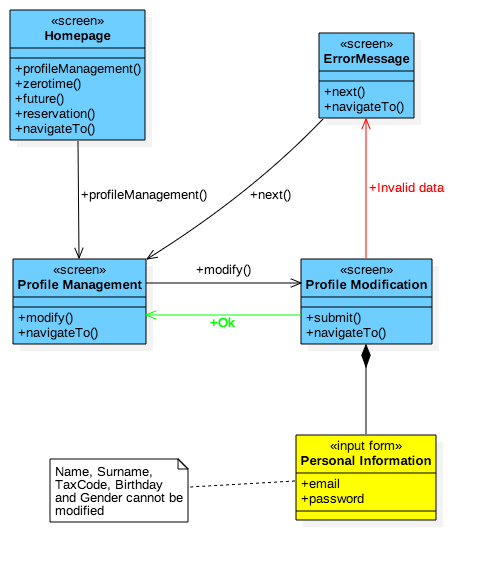
\includegraphics[width = \textwidth] {runtime/UX_ProfileManagement}
	\caption[UX Diagram for Profile Management.] {The UX diagram for the management of the personal profile. All the possible operations are displayed here.}
\end{figure}

\clearpage

\subsubsection{Zerotime and Future Rides}
\label{ArchitecturalDesign:UX_Ride}

\begin{figure}[hb!]
	\label{ArchitecturalDesign:fourthUX}
	\centering
	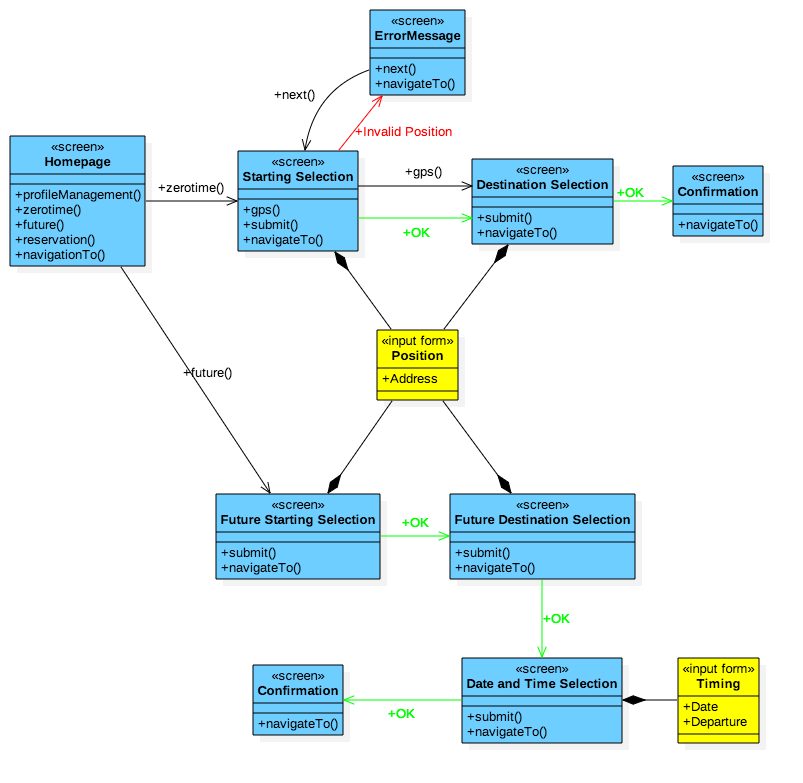
\includegraphics[width = \textwidth] {runtime/UX_Ride}
	\caption[UX Diagram for the Ride booking.] {The UX diagram for both the booking of a future ride and the asking for a zerotime ride, starting from the homepage.\\
		In order to make the diagram easy to understand, not all the error screens are inserted into the diagram: only the first one is shown.The other ones are similar and where there is an input form.}
\end{figure}

\clearpage

\subsubsection{Check The Reservations}
\label{ArchitecturalDesign:UX_CheckReservations}

\begin{figure}[hb!]
	\label{ArchitecturalDesign:thirdUX}
	\centering
	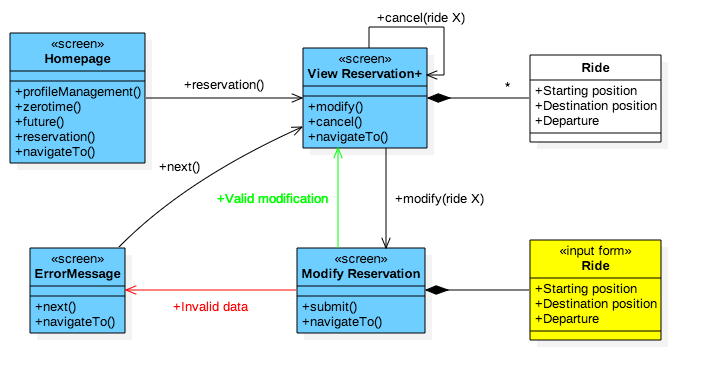
\includegraphics[width = \textwidth] {runtime/UX_CheckReservation}
	\caption[UX Diagram for Check the Reservations.] {The UX diagram for the management of the personal reservations.}
\end{figure}

%\clearpage

\subsubsection{Driver Functionalities}
\label{ArchitecturalDesign:UX_Driver}

\begin{figure}[hb!]
	\label{ArchitecturalDesign:fifthUX}
	\centering
	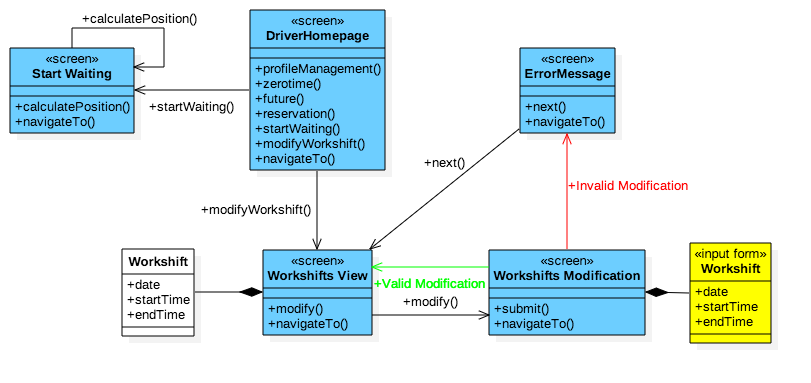
\includegraphics[width = \textwidth] {runtime/UX_Driver}
	\caption[UX Diagram for the Driver functionalities.] {The Ux diagram for the Driver functionalities.}
\end{figure}

\clearpage

\subsection{Sequence Diagram}
\label{ArchitecturalDesign:SD}

In this section are displayed the sequence diagram of myTaxiService run-view. In each diagram where the actor is an user and not a visitor of the website there is always an edge with \textquotedblleft Login Procedure\textquotedblright that can be misunderstood: the login to the websites it is required to perform the desired action, but if it is already done (for instance when the user is on his homepage after another operation) the login it is not requested again.\\

\subsubsection{Registration}
\label{ArchitecturalDesign:SD_Registration}

\begin{figure}[hb!]
	\label{ArchitecturalDesign:firstSD}
	\centering
	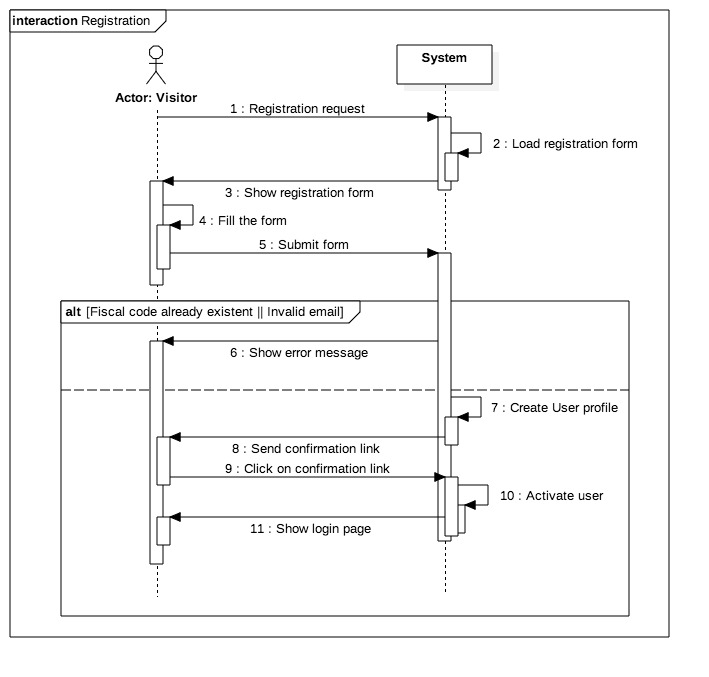
\includegraphics[width = \textwidth] {runtime/SD_Registration}
	\caption[Sequence Diagram for the Registration.] {The sequence diagram for the Registration.}
\end{figure}

\clearpage

\subsubsection{Login}
\label{ArchitecturalDesign:SD_Login}

\begin{figure}[hb!]
	\label{ArchitecturalDesign:secondSD}
	\centering
	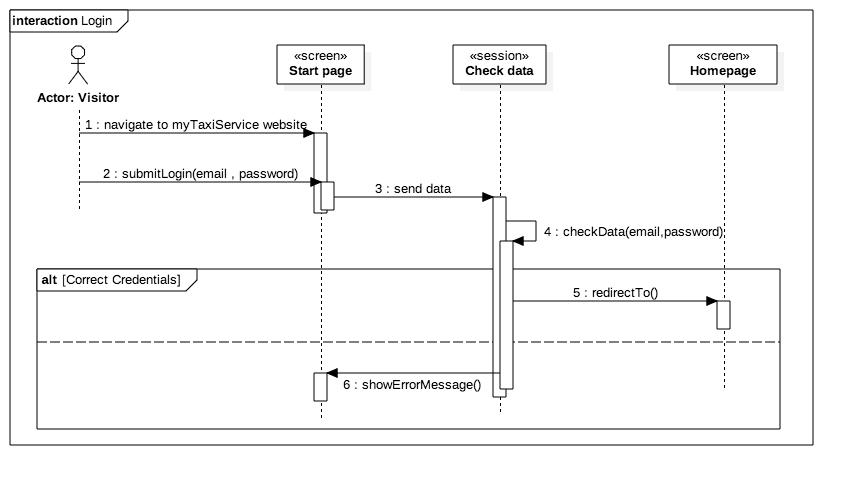
\includegraphics[width = 0.75\textwidth] {runtime/SD_Login}
	\caption[Sequence Diagram for the login.] {The sequence diagram for the Login.}
\end{figure}

%\clearpage

\subsubsection{Profile Management}
\label{ArchitecturalDesign:SD_ProfileManagement}

\begin{figure}[hb!]
	\label{ArchitecturalDesign:thirdSD}
	\centering
	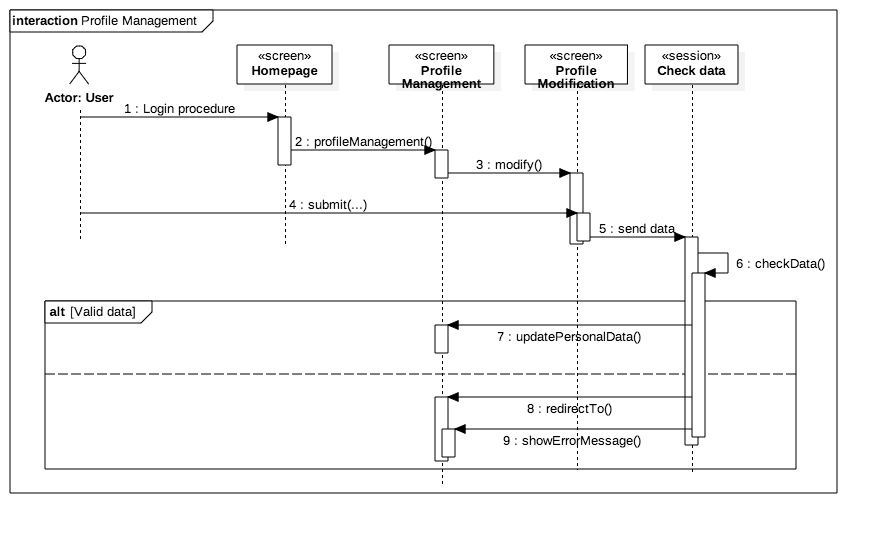
\includegraphics[width = 0.85\textwidth] {runtime/SD_ProfileManagement}
	\caption[Sequence Diagram for the Profile Management.] {The sequence diagram for the management of the personal profile.\\
		 The only data that can be modified are the email and the password used to log into the system, while name, surname, tax code, gender and birthday are not modifiable by definition.}
\end{figure}

\clearpage

\subsubsection{Check The Reservations}
\label{ArchitecturalDesign:SD_CheckReservation}

\begin{figure}[hb!]
	\label{ArchitecturalDesign:sixthSD}
	\centering
	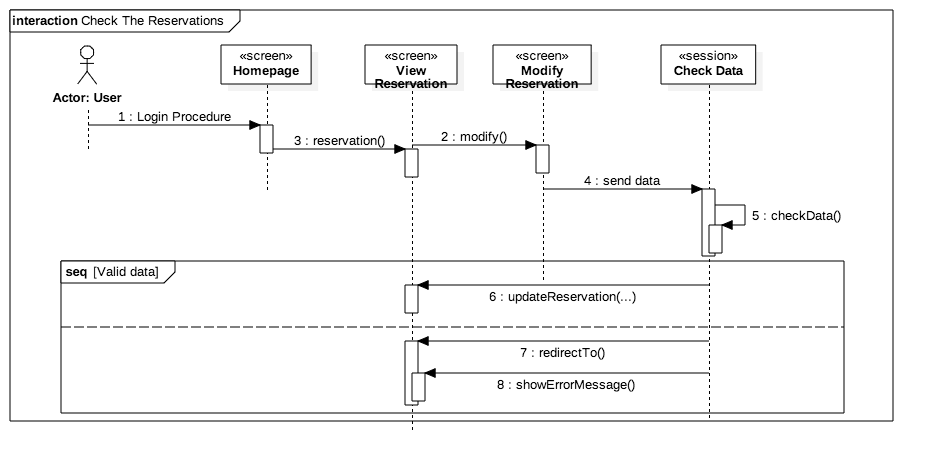
\includegraphics[width = 0.9\textwidth] {runtime/SD_CheckTheReservations}
	\caption[Sequence Diagram for Check the Reservations.] {The sequence diagram for the management of personal booking.}
\end{figure}

%\clearpage

\subsubsection{Start Waiting Time}
\label{ArchitecturalDesign:SD_StartWaitingTime}

\begin{figure}[hb!]
	\label{ArchitecturalDesign:fourthSD}
	\centering
	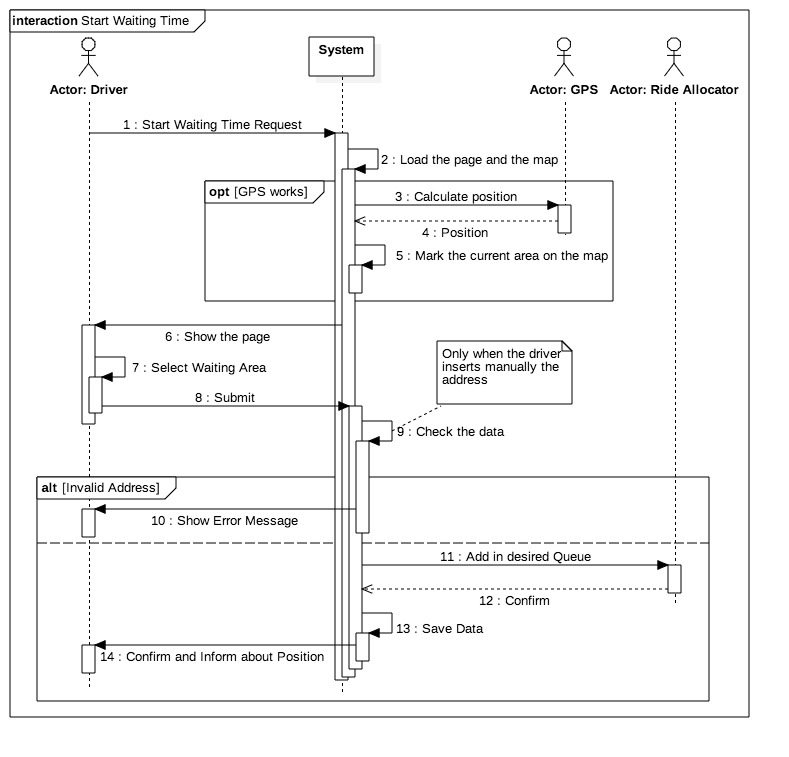
\includegraphics[width = 0.9\textwidth] {runtime/SD_StartWaitingTime}
	\caption[Sequence Diagram for Start Waiting Time.] {The sequence diagram for the notification of waiting time's start.}
\end{figure}

\clearpage

\subsubsection{Work shifts Management}
\label{ArchitecturalDesign:SD_WorkshiftsManagement}

\begin{figure}[hb!]
	\label{ArchitecturalDesign:fifthSD}
	\centering
	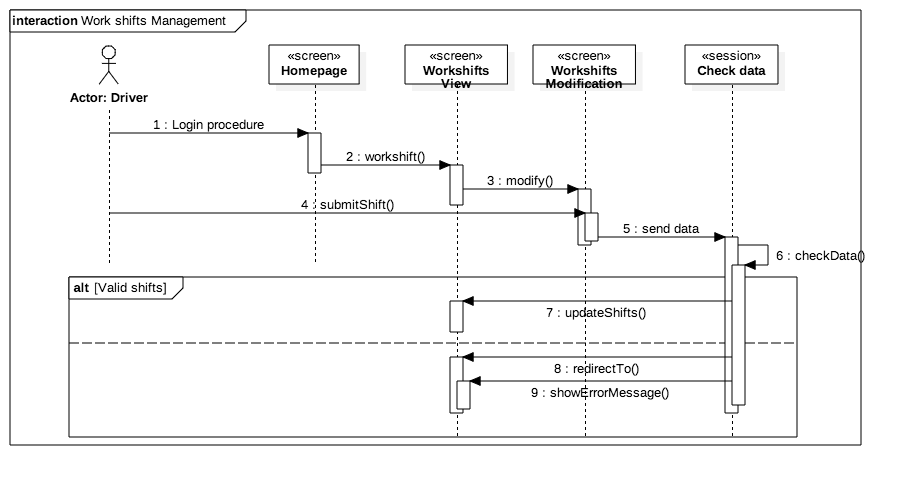
\includegraphics[width = 0.85\textwidth] {runtime/SD_WorkshiftsManagement}
	\caption[Sequence Diagram for the Work shifts Management.] {The sequence diagram for the management of the driver's work shifts.}
\end{figure}

%\clearpage

\subsubsection{Future Ride Booking}
\label{ArchitecturalDesign:SD_Zerotime}

\begin{figure}[hb!]
	\label{ArchitecturalDesign:seventhSD}
	\centering
	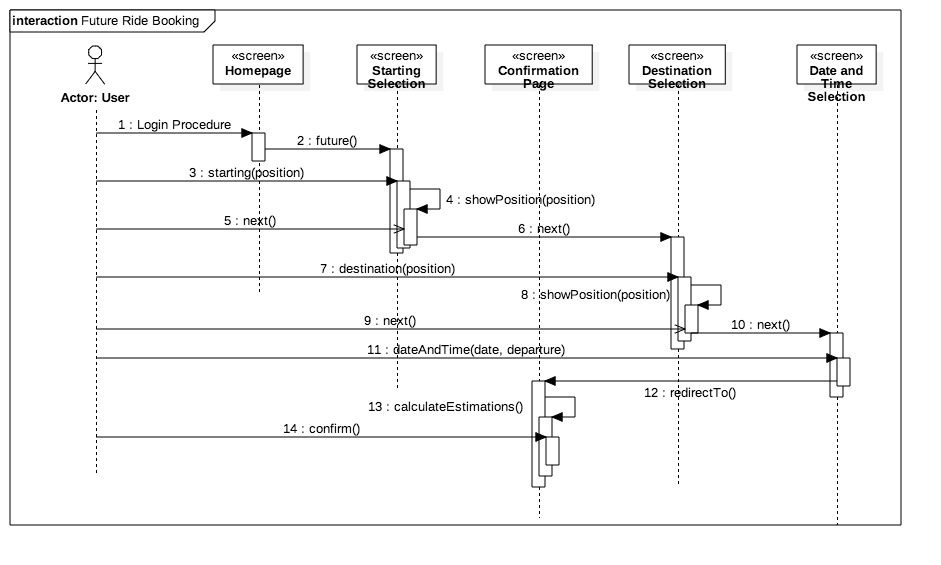
\includegraphics[width = 0.9\textwidth] {runtime/SD_FutureRideBooking}
	\caption[Sequence Diagram for the Future Ride.] {The sequence diagram for the booking of a future ride.\\
		In order to make the diagram easy to understand, the errors on inserting either the positions or the departure are not modelled.}
\end{figure}

\clearpage

\subsubsection{Zerotime Ride}
\label{ArchitecturalDesign:SD_Zerotime}

\begin{figure}[hb!]
	\label{ArchitecturalDesign:seventhSD}
	\centering
	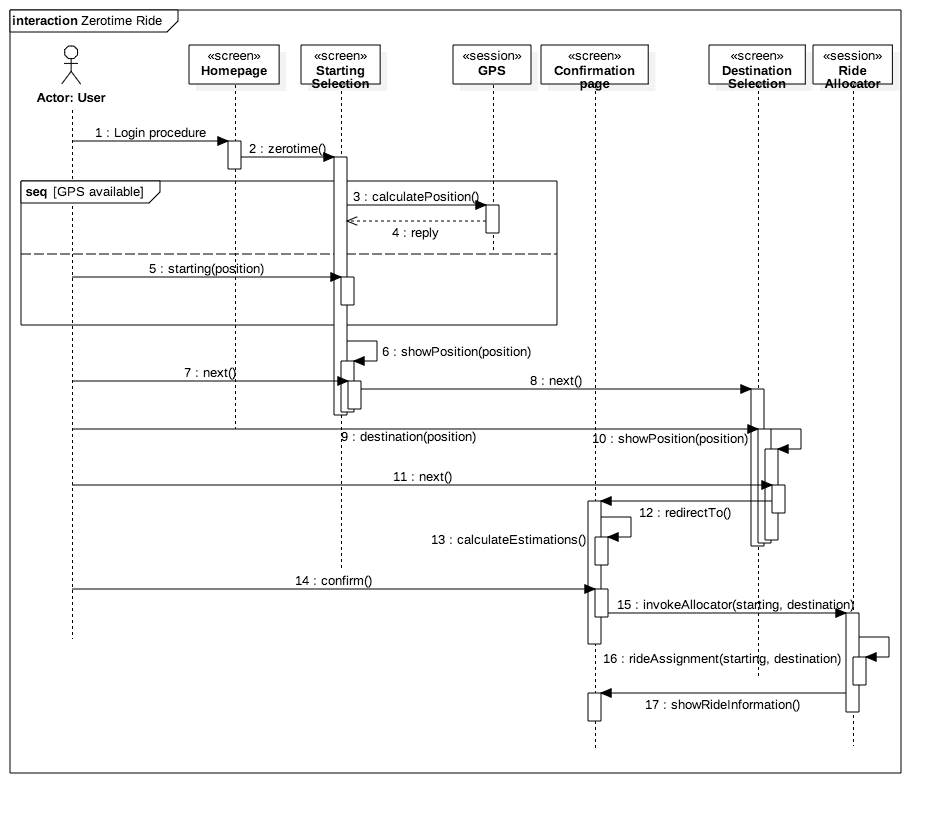
\includegraphics[width = \textwidth] {runtime/SD_ZerotimeRide}
	\caption[Sequence Diagram for the Zerotime Ride.] {The sequence diagram for the asking for a zerotime ride.\\
		In order to make the diagram easy to understand, the errors on inserting the positions are not modelled.}
\end{figure}

%\clearpage

\section{Component Interfaces}
\label{ArchitecturalDesign:comp_interfaces} 
This section describes the interfaces of the components, i.e. the operations they offer to the external world.\\
The methods are written in the following way:
\begin{center}
	\textit{return\textunderscore type method\textunderscore name ([parameter1\textunderscore type parameter1\textunderscore name], [\textellipsis])}
\end{center}

\begin{itemize}
	
	\item \textbf{GpsInterface}. This interface is implemented by the GPS system. For the GPS functionality we use also the Google APIs to obtain the address corresponding to a gps position and to show the map.\\
	The GpsInterface offers two public methods:
	\begin{itemize}
		\item \textit{Position calculatePosition()}\\
		it calculates the current position of the method's caller and return an object of type Position.
		\item \textit{double getGpsLatitude(Position pos)}\\
		it returns a double precision decimal number that represents the latitude of the Position given as parameter.
	\end{itemize}
	\begin{itemize}
		\item \textit{double getGpsLongitude(Position pos)}\\
		it returns a double precision decimal number that represents the longitude of the Position given as parameter
	\end{itemize}
	
	\item \textbf{RideAllocatorInterface}. This interface is implemented by the Ride Allocator to manage the rides and the queues of available drivers for each area. It offers three public methods:
	\begin{itemize}
		\item \textit{void assignRide(Ride ride, Driver driver)}\\
		it assigns Ride given as first parameter to the Driver, given as second parameter.
		\item \textit{void enqueueDriver(Driver driver, Position pos)}\\
		it calculates the Area which the Position of the driver (given as a second parameter) belongs to, then it add the Driver (given as first parameter) to the corresponding queue of available drivers of the area.
		\item \textit{boolean isValidAddress(String city, String street)}\\
		it verifies the existence of the address, given as the couple of String(s) representing the city and the street, in one of the areas covered by myTaxyService. It returns the boolean value true if the address exists, false otherwise.
	\end{itemize}	
	
	\item \textbf{ClientAndUsersHandlerInterface}. This interface is implemented by the Client and Users handler and offers the public methods to manage the user functionalities:
	\begin{itemize}
		\item \textit{String login(String email, String password)}\\
		this method needs two parameters: a String containing the e-mail of the user and a String containing the encrypted password with the method defined by the SecurityManagerInterface. It returns a String representing the result of the operation with a number identifier at starting and a text message after. All the possible results are:
		\begin{itemize}
			\item \textit{\textquotedblleft 0 : Login Successful\textquotedblright}
			\item \textit{\textquotedblleft 1 : User already logged in"}
			\item \textit{"2 : Login Error, the e-mail and/or the password are wrong"}
		\end{itemize}
		
	\end{itemize}
	\begin{itemize}
		\item \textit{public String register(String email, String password, String name, String surname, String taxCode, Date birthday, String cityOfResidence)}\\
		this method needs many String parameters: the e-mail of the user, the encrypted password with the method defined by the SecurityManagerInterface, the name, surname, personal tax code, birthday, the city of residence. It returns a String representing the result of the operation with a number identifier at starting and a text message after. All the possible results are:
		\begin{itemize}
			\item \textit{"0 : Registration Successful, an e-mail with activation code has been sent"}
			\item \textit{"1 : Registration Error, user already registered with that tax code"}
			\item \textit{"2 : Registration Error, e-mail already in use"}
			\item \textit{"3 : Registration Error, data are not valid"}	
		\end{itemize}
		
	\end{itemize}	
	
	\item \textbf{SecurityManagerInterface}. This interface is implemented by the Security Manager and offers these public methods:
	\begin{itemize}
		\item \textit{String encryptPassword(String password)}\\
		it encrypts a password given as a String parameter, with the hashing method estabilished by the security rules of the system, and returns the result.
	\end{itemize}	
	
	\item \textbf{DBMSInterface}. This interface is implemented by the DBMS and offers general public methods to access the data of the database:
	\begin{itemize}
		\item \textit{Object getValue(String key, String from, String whereCondition)}
		gets the value corresponding to a specific key of a record in the database. The first parameter is the name of the key of which we want to know the corresponding value, for a specific record. The second parameter is the name of the table to retrieve data from or a join of tables. The third parameter is a part of SQL query containing the conditions to search the desired record.\\
		The method returns the Object representing the value corresponding to the specific key of the desired record. If there are more than one records according to the whereCondition (third parameter) only the first record is taken.
		
		\item \textit{Object[] getValue(String[] keys, String from, String whereCondition)}
		this is an overload method similar to the one above, but it returns an array of Object(s) corresponding to the values of the keys in the array of String(s) given as first parameter. The meaning of the other parameters is the same of the method above. Again if there are more than one records according to the whereCondition (third parameter) only the first record is taken.
		
		\item \textit{Object[][] getAllValues(String[] keys, String from, String whereCondition)}
		this method is similar to the one above, but it returns all the values corresponding to the specific keys of all the records that respect the whereCondition (third parameter), not only the first record as it was above instead. The meaning of the parameters is the same of the method above. This method returns a matrix of Object(s) which contains all the records as rows and all the values corresponding to the keys as columns, in the same order of the array of keys given as second parameter.
		
		\item \textit{void setValue(String key, String value, String from, String whereCondition)}
		sets the value of a specific key of any record in the database that respect the whereCondition parameter. The first parameter is the name of the key of which we want to set the value, given as second parameter, for a specific record. The third parameter is the name of the table or a join of tables, where the desired key is. The fourth parameter is a part of SQL query containing the conditions to search the desired record.
	\end{itemize}
		
	
\end{itemize}



\section{Selected architectural styles and patterns}
\label{ArchitecturalDesign:design_patterns}
For myTaxyService we have chosen to follow two fundamental architectural patterns combined, Model-View-Controller (also called MVC) and Service-Oriented Architecture (also called SOA).\\
The pattern MVC, as its name says, consists in the clear division between three main interconnected software parts, so as to separate internal representations of information from the ways that information is presented to or accepted from the user. The three parts are:
\begin{itemize}
	\item \textit{Model.} It represents the underlying, logical structure of data in a software application and the high-level class associated with it. The Model does not contain any information about the user interface.\\
	It communicates with the Controller, which can read or modify the data contained. The only interaction with the View is the notification of the data changing in some applications of MVC pattern.
	
	\item \textit{View.} It is a collection of classes representing the elements in the user interface (all of the things the user can see and respond to on the screen, such as buttons, display boxes, and so forth). Usually the View is generalized and made extensible with the use of an interface with public methods, implemented by different view implementations for various user interfaces.\\
	The View doesn't contain any information of the real data contained in the Model, it knows only the information that receives from the Controller and sends to user input to it.
	
	
	\item \textit{Controller.} It represents the bridge between the Model and the View, and is used to communicate between their classes. It receives the user inputs from the View and as consequence retrieves or modifies the data contained in the Model. It contains information of the Model and of the View and knows how to interact with them.\\
\end{itemize}

A Service-Oriented Architecture is composed of three parts:
\begin{itemize}
	\item \textit{Service requestor.} It  requests the execution of a service. It asks for a service contained in the Service registry and once that is found, the Service requestor is bound to the correct service offered by the Service provider. 
	\item \textit{Service provider.} It offers services. It publish all the available services with their description in the public Service registry and when receives a request it bind the requestor with the correct service.
	\item \textit{Service registry.} It provides information about all the available services.
\end{itemize}

Our application and adaptation of MVC and SOA for myTaxyService, is fully described before in \autoref{ArchitecturalDesign:high_level}.\\
\\
According to the class diagram presented in the RASD, we have chosen to follow also some design patterns, such as the Factory Pattern and Singleton.\\
The \textit{Factory Pattern} consists in the creation of objects without exposing the creation logic to the client and referring to newly created object using a common interface or super class. In the Factory Pattern a specific class (a Factory class) offers public methods to create objects using a common interface or abstract class and it knows the creation logic of the concrete implementation of the common interface. The client that calls the factory methods (the methods used to create objects) of the factory class, passing a parameter identifier of the required object, don't know the real creation logic of the object, they knows only the Factory class and its factory methods and the common interface or abstract class which the desired object belongs to.\\
In the case of myTaxyService we use this pattern to create a User of a specific type (Driver or normal User) and also a Ride of a specific type (zerotime or future ride), without knowing in fact the real create logic of the users and rides depending by the type of them. There will be a factory class for the users and one for the rides that know the real create logic of them.\\
\\
The \textit{Singleton Pattern} involves a single class which is responsible to create an object while making sure that only single object gets created. This class provides a way to access its only object which can be accessed directly without need to instantiate the object of the class. The constructor of the class is hidden to the external world to make sure that the only way that an instance of the object can be obtained is by a static method of the class that doesn't create more than one instance of its object.\\
We use the Singleton pattern for the internal components of the Provider to make sure that have always only one instance of them and they can be easily accessible with a static method. (for more information about the provider see \autoref{ArchitecturalDesign:provider}).

%End of chapter
\end{document}